%!TEX program = xelatex
% 完整编译: xelatex -> biber/bibtex -> xelatex -> xelatex
\documentclass[lang=cn,11pt,a4paper]{elegantpaper}

\title{有限元第二次编程作业}
\author{W Huang}
\date{\zhtoday}


% 本文档命令
\usepackage{array}
\usepackage{float}
\usepackage{multirow}
\usepackage{amsmath}
\usepackage{amssymb}
\newcommand{\ccr}[1]{\makecell{{\color{#1}\rule{1cm}{1cm}}}}

\begin{document}

\maketitle

\section{编程第一题}

\subsection{求解设置}

求解PDE
\begin{equation}
    \left\{
        \begin{array}{l}
            -\Delta u = f,\quad \text{in}\;\Omega=(0,1),\\
            u(0) = u(1) = 0.
        \end{array}
    \right.
\end{equation}

取一右端项 $f\in L_\text{loc}^2(\Omega)$:
\begin{equation}
    f(x)=\frac{1}{x}.
\end{equation}

显然 $f$ 在 $0$ 处不连续,且 $f\notin L^2(\Omega)$。我们导出精确解:
\begin{equation}
    u(x)=x\ln x.
\end{equation}

注意到 $u\in H^1(\Omega)\cap C(\overline{\Omega})$。
使用非均匀网格$x_i=(i/N)^2$,取$\mathcal{P}_1$元。
使用预优共轭梯度法 (Preconditioned CG) 求解,
用超松弛迭代 (SSOR) 作为预优因子,
超松弛系数取 $2-\varepsilon$,其中 $\varepsilon=10^{-12}$。
右端项的数值积分由一阶高斯求积公式计算。

\subsection{编译说明}

请安装 deal.ii 及其依赖库,见 https://www.dealii.org/developer/readme.html;安装完毕后,在本文档目录下打开终端,依次运行:
\begin{lstlisting}
cd src-p1
mkdir build
cd build
cmake ..
make release
make
\end{lstlisting}
等待编译完成后,用以下命令执行测试:
\begin{lstlisting}
./elliptic 10 u
\end{lstlisting}
上述测试采用 1.1 节所述的非均匀网格,规模为 $N=2^{10}$,如果需要改变网格规模,将 \verb|10| 换成别的正整数即可。另外,如果想测试均匀网格,只需将上述命令中的 \verb|u| 删去即可。

\subsection{数值结果}

\begin{figure}[H]
    \centering
    \begin{minipage}[t]{0.48\textwidth}
        \centering
        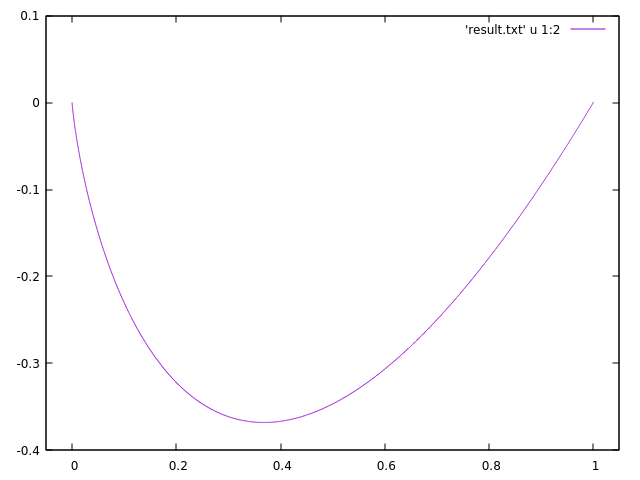
\includegraphics[width=0.9\linewidth]{png/p1-solution}
        \caption{\small $N=2^{14}$ 时非均匀网格的数值解 $u_h$}
    \end{minipage}
    \hspace{1em}
    \begin{minipage}[t]{0.48\textwidth}
        \centering
        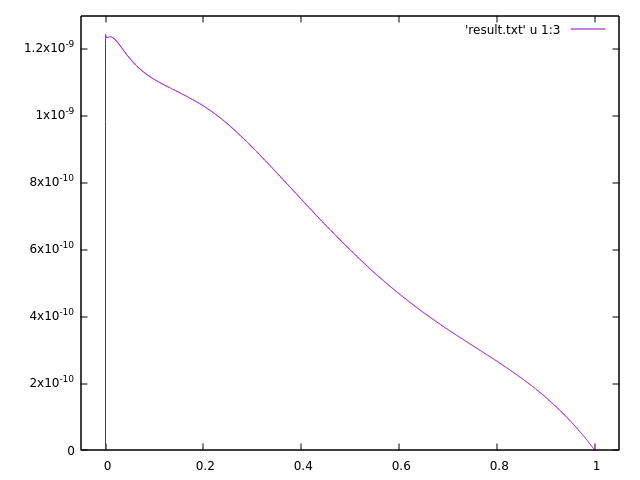
\includegraphics[width=0.9\linewidth]{png/p1-error}
        \caption{\small $N=2^{14}$ 时非均匀网格的误差 $u_h-u$}
    \end{minipage}
\end{figure}

可以看到,误差集中在奇异点附近。

\begin{table}[H]
    \centering
    \begin{tabular}{|c|c|c|c|c|c|c|c|}
    \hline
    单元数量                    & $2^{14}$ & 阶数 & $2^{15}$ & 阶数 & $2^{16}$ & 阶数 & $2^{17}$ \\ \hline
    $||u-u_h||_{L_2}$      & 1.90e-09     & 1.92 & 5.02e-10     & 1.51 & 1.76e-10     & 2.16 & 3.95e-11     \\ \hline
    $||u-u_h||_{L_\infty}$ & 2.91e-09     & 2.00 & 7.30e-10     & 1.59 & 2.42e-10     & 1.18 & 1.07e-10     \\ \hline
    $||u-u_h||_{H_1}$      & 1.60e-04     & 0.96 & 8.24e-05     & 0.96 & 4.25e-05     & 0.96 & 2.19e-05     \\ \hline
    CG 迭代次数            & 14 & & 16 & & 17 & & 19\\    
\hline
    装配耗时 (s)           & 0.019         &      & 0.035          &      & 0.072           &      & 0.15     \\ \hline
    求解耗时 (s)           & 0.0051         &      & 0.010          &      & 0.024           &      & 0.048     \\ \hline
    \end{tabular}
    \caption{\small 预优共轭梯度法,预优因子:SSOR,超松弛系数:$2-\varepsilon\;(\varepsilon=10^{-12})$。}
\end{table}

由于网格尺寸太细,在机器精度的限制下,$L_2$ 和 $L_\infty$ 范数已经无法继续下降。另外可以看到,SSOR 作为预优因子效果非常好,随着网格加密,CG 迭代次数基本不会增加。换言之,当超松弛系数趋近于 $2$ 时,在 SSOR 的作用下,迭代矩阵的条件数与网格尺寸几乎无关。

刚度矩阵条件数(二范数下)的数值结果如下,数值结果支持 $\kappa(A)\sim O(N^3)$:

\begin{table}[H]
    \centering
    \begin{tabular}{|c|c|c|c|c|c|c|c|}
    \hline
    单元数量                    & $256$ & 阶数 & $512$ & 阶数 & $1024$ \\ \hline
  $\kappa(A)$            & 1.93116e+06 & 2.99 & 1.53591e+07 & 3.00 & 1.22513e+08\\    \hline
    \end{tabular}
    \caption{\small 刚度矩阵的二范数条件数,即 $\kappa(A)=||A||_2\cdot ||A^{-1}||_2$。}
\end{table}

为了测试刚度矩阵的条件数对求解性能的影响,我们不使用预优因子再进行一次测试。与预优 CG 相比,朴素 CG 的求解性能大大降低,我们只好将网格规模减小以进行测试。

\begin{table}[H]
    \centering
    \begin{tabular}{|c|c|c|c|c|c|c|c|}
    \hline
    单元数量                    & $2^{12}$ & 增长率 & $2^{13}$ & 增长率 & $2^{14}$ \\ \hline
    CG 迭代次数            & 42996 & 2.86 & 122781 & 2.85 & 350164\\    
\hline
    装配耗时 (s)           & 0.005          &      & 0.01           &      & 0.02     \\ \hline
    求解耗时 (s)           & 0.49          &      & 2.35           &      & 12.7     \\ \hline
    \end{tabular}
    \caption{\small 朴素共轭梯度法。}
\end{table}

\appendix
%\appendixpage
\addappheadtotoc

\end{document}
